\documentclass[14pt]{article}
\usepackage{../../report-tex/styles}
\usepackage{graphicx}


\begin{document}

    \titlewithlabnum{6}

    \tableofcontents
    \newpage


    \section{Мета:}
    Мета роботи: отримати вміння та навички використовувати засоби обміну інформацією та запрограмувати взаємодію незалежно працюючих програмних компонентів


    \section{Завдання:}
    \begin{enumerate}
        \item    Вимоги щодо організації системи Для виконання лабораторної роботи потрібно створити три незалежні програми, для чого можна створити три проекта у одному рішенні (Solution) Microsoft Visual Studio C++. У цьому випадку усі виконувані файли будуть знаходитися у спільній папці \{ \}Debug або \{ \}Release. Головний проект – програма Lab6 має бути менеджером, який керує двома іншими програмами – Object2 та Object3. Програма Lab6 повинна автоматично, без участі користувача налагоджувати співпрацю та виконувати обмін повідомленнями з програмами Object2 та Object3 для виконання потрібного завдання згідно наведеному вище алгоритму. У кожній програмі передбачити автоматичну обробку потрібних повідомлень і переходів з одного стану в інший. Далі вимоги щодо функціонування системи об'єктів.
        \item    1. Для початку роботи користувач програми вибирає потрібний пункт меню програми Lab6. Далі з’являється вікно діалогу, у якому потрібно ввести параметри згідно варіанту завдання. У вікні діалогу користувач натискує кнопку "Так" (або "Виконати") і на цьому місія користувача закінчується – далі він тільки спостерігає, як програма сама автоматично виконає усе, що потрібно для отримання результату. Виклик інших програм – Object2 та Object3 головна програма Lab6 повинна робити без участі користувача.
        \item    2. Обмін повідомленнями та масивами даних між програмами Lab6, Object2 та Object3 повинен відбуватися автоматично, без участі користувача. Програма Lab6 повинна автоматично у певній послідовності знаходити та викликати програми Object2 та Object3.
        \item    3. У результаті одного сеансу роботи користувач повинен бачити головні вікна програм Object2 та Object3, у яких відображатимуться потрібні результати відповідно варіанту завдань. Для цього вікна програм повинні автоматично розташуватися так, щоб усі результати було видно. Програма Lab6 повинна залишатися у активному стані, щоб користувач мав можливість повторно виконати роботу.
        \item    4. Передбачити варіанти успішної роботи у випадках, коли програми Object2 та Object3 (одна або обидві) до того вже були викликані.
        \item    5. По завершенні роботи програми Lab6 повинні автоматично завершуватися і програми Object2 та Object3.
    \end{enumerate}

    \begin{align}
        G &= (22) \bmod 4 = 2
    \end{align}

    \subsection{Варіант 2:}
    \begin{enumerate}
        \item \begin{enumerate}
                  \item    Користувач вводить значення n, Min, Max у діалоговому вікні.
                  \item    Програма викликає програми Object2, 3 і забезпечує обмін повідомленнями для передавання та отримання інформації.
                  \item    Створює вектор n дробових (double) чисел у діапазоні Min – Max
        \end{enumerate}
        \item \begin{enumerate}
                  \item    Створює вектор n дробових (double) чисел у діапазоні Min – Max
                  \item    Показує числові значення у декількох стовпчиках та рядках у власному головному вікні
                  \item    Записує дані в Clipboard Windows у текстовому форматі
        \end{enumerate}
        \item \begin{enumerate}
                  \item    Зчитує дані з Clipboard Windows
                  \item    Виконує сортування масиву чисел і відображає його у декількох стовпчиках та рядках у власному головному вікні
        \end{enumerate}
    \end{enumerate}


    \section{Текст програми:}
    \subsection{Module: com.github.erotourtes.drawing.editor}
\lstinputlistingukr{DmProcessor.kt}{../src/main/kotlin/com/github/erotourtes/drawing/editor/DmProcessor.kt}
\lstinputlistingukr{Editor.kt}{../src/main/kotlin/com/github/erotourtes/drawing/editor/Editor.kt}
\lstinputlistingukr{Editors.kt}{../src/main/kotlin/com/github/erotourtes/drawing/editor/Editors.kt}
\lstinputlistingukr{ShapesList.kt}{../src/main/kotlin/com/github/erotourtes/drawing/editor/ShapesList.kt}

\subsection{Module: 1.0}
\lstinputlistingukr{MANIFEST.MF}{../src/main/resources/META-INF/MANIFEST.MF}

\subsection{Module: com.github.erotourtes.view}
\lstinputlistingukr{MainController.kt}{../src/main/kotlin/com/github/erotourtes/view/MainController.kt}
\lstinputlistingukr{MainView.kt}{../src/main/kotlin/com/github/erotourtes/view/MainView.kt}
\lstinputlistingukr{MenuBar.kt}{../src/main/kotlin/com/github/erotourtes/view/MenuBar.kt}
\lstinputlistingukr{ToolBar.kt}{../src/main/kotlin/com/github/erotourtes/view/ToolBar.kt}

\subsection{Module: com.github.erotourtes.app}
\lstinputlistingukr{MyApp.kt}{../src/main/kotlin/com/github/erotourtes/app/MyApp.kt}

\subsection{Module: com.github.erotourtes.drawing}
\lstinputlistingukr{CanvasPane.kt}{../src/main/kotlin/com/github/erotourtes/drawing/CanvasPane.kt}
\lstinputlistingukr{EditorHandler.kt}{../src/main/kotlin/com/github/erotourtes/drawing/EditorHandler.kt}

\subsection{Module: com.github.erotourtes.drawing.shape}
\lstinputlistingukr{Shape.kt}{../src/main/kotlin/com/github/erotourtes/drawing/shape/Shape.kt}
\lstinputlistingukr{Shapes.kt}{../src/main/kotlin/com/github/erotourtes/drawing/shape/Shapes.kt}

\subsection{Module: com.github.erotourtes.styles}
\lstinputlistingukr{ToolbarStyles.kt}{../src/main/kotlin/com/github/erotourtes/styles/ToolbarStyles.kt}

\subsection{Module: com.github.erotourtes.utils}
\lstinputlistingukr{Dimension.kt}{../src/main/kotlin/com/github/erotourtes/utils/Dimension.kt}
\lstinputlistingukr{ExtensionFunctions.kt}{../src/main/kotlin/com/github/erotourtes/utils/ExtensionFunctions.kt}
\lstinputlistingukr{Utils.kt}{../src/main/kotlin/com/github/erotourtes/utils/Utils.kt}




    \section{Ілюстрації:}
    \begin{figure}[H]
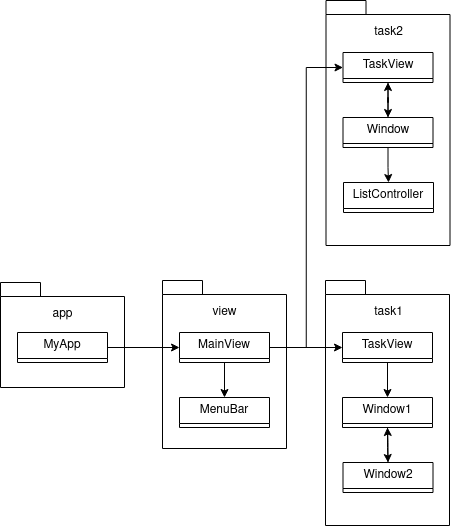
\includegraphics[width=10cm]{1}
\centering
\end{figure}



    \section{Висновки:}
    Отже, я отримав вміння та навички використання обміну інформацією та запрограмував взаємодію незалежно працюючих програмних компонентів

\end{document}
